% !TEX program = pdflatex
\documentclass[11pt]{article}
\usepackage{amsmath, amssymb, amsfonts}
\usepackage{graphicx}
\usepackage{geometry}
\usepackage{hyperref}
\usepackage{float}
\usepackage{xcolor}
\usepackage{listings}
\lstset{
    language=Python,
    basicstyle=\ttfamily\small,
    keywordstyle=\color{blue}\bfseries,
    stringstyle=\color{red},
    commentstyle=\color{gray}\itshape,
    numberstyle=\tiny\color{gray},
    numbers=left,
    numbersep=5pt,
    showstringspaces=false,
    frame=single,
    breaklines=true
}
\geometry{margin=1in}
\title{Module Example Assignment\\\large Chapter X, Sections Y-Z}
\author{Your Name}
\date{Date Assignment is Due}
\begin{document}
\maketitle

\section*{Problem Set}
\textbf{X.Y.1 Some exercise from the textbook that likely has inline latex like $\boldsymbol{\int_0^{\infty} e^{-x} \,dx}$.}

The answer to the exercise generally has inline latex as well like $\int_0^{\infty} e^{-x} \,dx$. Often times there are lines like the following which are all LaTeX,
\begin{align*}
    \int_0^{\infty} e^{-x} \,dx & = {\left[-e^{-x} \right]}_0^{\infty}       \\
                                & = \lim_{x \to \infty} (-e^{-x}) - (-e^{0}) \\
                                & = 0 - (-1) = 1.
\end{align*}

\pagebreak

\section*{Software Assignment}
\textbf{Some prompt assigned as a software assignment. For example, create a visualization representing $\boldsymbol{\int_0^{\infty} e^{-x} \,dx}$.}

\begin{figure}[H]
    \centering
    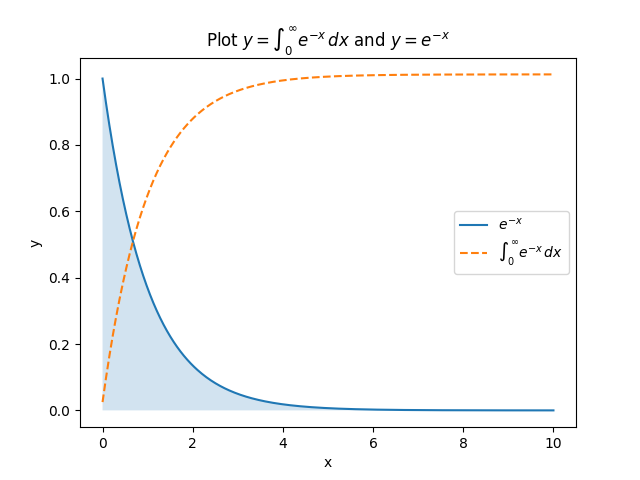
\includegraphics[width=0.95\textwidth]{software-assignment.png}
    \caption{Visualization of $e^{-x}$ and its integral approximation.}
\end{figure}

\pagebreak

\noindent Below is the Python code used to generate the figure:

\lstinputlisting[language=Python]{main.py}

\end{document}
